\chapter{网络编程上}
\noindent\textbf{课前思考:}
\begin{enumerate}
	\item 如何把互联网上网页抓取下来?
	\item 如何与互联网上网络资源通信?
	\item 如何在两个Java程序之间建立网络连接?
	\item 面向连接与非面向连接的通信方式有什么区别?
\end{enumerate}
\textbf{学习目标:}理解计算机网络编程的概念,掌握如何使用Java在一台或多台计算机之间
进行基于TCP/IP协议的网络通讯。
\par 通过理解TCP/IP协议的通讯模型,以JDK提供的java.net包为工具,掌握各种基于Java的
网络通讯的实现方法。
\\ \textbf{难点和重点:}
\begin{enumerate}
	\item 基于URL的网络编程
	\item 基于TCP的C/S网络编程
	\item 基于UDP的C/S网络编程
\end{enumerate}

\section{URL对象}
\subsection{网络基础知识}
\begin{itemize}
	\item IPV4地址(32位,4字节)
	\item IPV6地址(128位,16字节)
	\item 主机名(hostname)
	\item 端口号(port number)
	\item 服务类型(service):http、telnet、ftp、smtp
\end{itemize}
\subsection{通过URL读取WWW信息}
\begin{lstlisting}[language=java]
public class URLReader {
	public static void main(String[] args) {
		URL cs = null;
		BufferedReader in = null;
		try {
			cs = new URL("http://www.sina.com/");
			in = new BufferedReader(new InputStreamReader(cs.openStream()));
			String inputLine;
			while ((inputLine = in.readLine()) != null) {
			System.out.println(inputLine);
			}
			in.close();
		} catch (IOException e) {
			e.printStackTrace();
		}
	}
}
\end{lstlisting}
\subsection{URL类}
\noindent URL(Uniform Resource Locator)一致资源定位器的简称,表示Internet上某一资源的地址。
\\ URL组成:Protocol:resourceName
\par 协议名指明获取资源所使用的传输协议,如http、ftp、gopher、file等,
资源名则应该是资源的完整地址,包括主机名、端口号、文件名或文件内部的一个引用。
\subsection{构造URL对象}
\begin{itemize}
	\item public URL(String spec)
	\subitem URL urlBase = new URL("http://gamelan.com/");
	\item public URL(URL context, String spec)
	\subitem URL gamelan = new URL("http://gamelan.com/pages/");
	\subitem URL gamelanGames = new URL(gamelan, "Gamelan.game.html");
	\subitem URL gamelanNetwork = new URL(gamelan, "Gamelan.net.html");
	\item public URL(String protocol, String host, String file);
	\item public URL(String protocol, String host, int port, String file);
\end{itemize}
\subsection{获取URL对象属性}
\begin{itemize}
	\item public String getProtocol()
	\item public String getHost()
	\item public String getPort()
	\item public String getFile()
	\item public String getRef()
\end{itemize}
\section{URL Connection对象}
\subsection{URL Connection}
\noindent 一个URL Connection对象代表一个URL资源与Java程序的通讯连接,可以通过它对这个URL资源读或写
\\ 与URL的区别
\begin{itemize}
	\item 一个单向,一个双向;
	\item 可以查看服务器的响应消息的首部;
	\item 可以设置客户端请求的首部;
\end{itemize}
使用URL Connection通信一般步骤:
\begin{enumerate}
	\item 构造一个URL对象;
	\item 调用URL对象的openConnection()方法获取对应该URL的URL Connection对象;
	\item 配置URL Connection对象;
	\item 读取首部字段;
	\item 获得输入流读取数据;
	\item 获得输出流写入数据;
	\item 关闭连接。
\end{enumerate}
\section{Get请求与Post请求}
\subsection{发送Get请求}
\begin{lstlisting}[language=java]
public static String sendGet(String url, String param){
	String result = "";
	BufferedReader in = null;
	String urlName = url + "?" + param;
	try {
		URL realUrl = new URL(urlName);
		URLConnection con = realUrl.openConnection();
		con.setRequestProperty("accept", "*/*");
		con.setRequestProperty("connection", "Keep-Alive");
		con.connect();
		in = new BufferedReader(new InputStreamReader(con.getInputStream()));
		String line;
		while ((line = in.readLine()) != null) {
			result += line;
		}
	} catch (Exception e) {}
	finally {
		try{
			if (in != null) {
				in.close();
			}
		} catch (Exception ex){}
	}
	return result;
}
\end{lstlisting}
\subsection{发送POST请求}
POST请求的参数通过URL Connection的输出流写入参数。
\begin{lstlisting}[language=java]
public static String sendPost(String url, String param){
	PrintWriter out = null;
	String result = "";
	BufferedReader in = null;
	try {
		URL realUrl = new URL(url);
		URLConnection con = realUrl.openConnection();
		con.setRequestProperty("accept", "*/*");
		con.setRequestProperty("connection", "Keep-Alive");
		con.setDoOutput(true);
		out = new PrintWriter(con.getOutputStream());
		out.print(param);
		out.flush();
		in = new BufferedReader(new InputStreamReader(con.getInputStream()));
		String line;
		while ((line = in.readLine()) != null) {
			result += line;
		}
	} catch (Exception e) {}
	finally {
		try{
			if (in != null) {
			in.close();
		}
		if (out != null) {
			out.close();
		}
		} catch (Exception ex){}
	}
	return result;
}
\end{lstlisting}
\subsection{HttpURLConnection类}
在URLConnection的基础上提供了一系列针对http请求的内容
\begin{itemize}
	\item HTTP状态码
	\item setRequestMethod(GET/POST)
	\item getResponseCode(获取HTTP的响应)
\end{itemize}
\section{Socket通信原理}
\subsection{TCP传输协议}
TCP(Transport Control Protocol): 面向连接的能够提供可靠的流式数据传输的协议。
\par 如java中的URL、URLConnection、Socket、ServerSocket等都使用TCP协议通讯。
\subsection{socket通讯}
网络上的两个程序通过一个双向的通讯连接实现数据的交换,这个双向链路的一段称为一个socket。
\\socket通常用来实现客户方和服务方的连接。
\begin{figure}[!h]
	\centering
	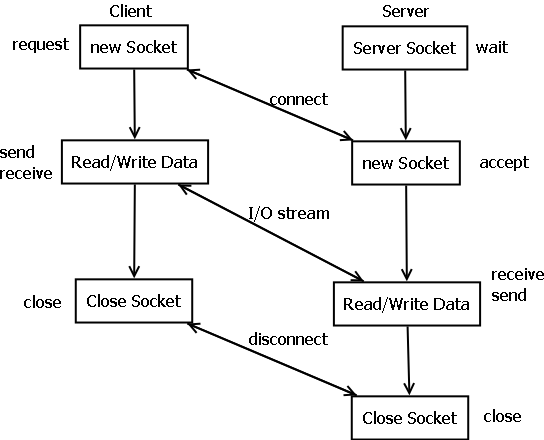
\includegraphics[width=0.8\textwidth]{image/socket.png}
	\caption{Socket通信原理}
\end{figure}
\section{Socket通信实现}
\subsection{创建socket}
\begin{itemize}
	\item Socket()
	\item Socket(InetAddress address, int port)
	\item Socket(String host, int port)
	\item Socket(InetAddress host, int port, InerAddress localAddr,int localPort)
	\item Socket(String host, int port, InetAddress localAdde, int localPort)
\end{itemize}
\subsection{客户端Socket的建立}
\begin{lstlisting}[language=java]
try {
	Socket socket = new Socket("127.0.0.1", 2000);
} catch (IOException e) {
	System.out.println("Error: " + e);
}
\end{lstlisting}
\subsection{服务端Socket的建立}
\begin{lstlisting}[language=java]
ServerSocket server = null;
try {
	server = new SocketServer(2000);
} catch (IOException e) {
	System.out.println("can not listen to: " + e);
}
Socket socket = null;
try {
	socket = server.accept();
} catch (IOException e) {
	System.out.println("Error: " + e);
}
\end{lstlisting}
\subsection{打开输入/输出流}
\begin{lstlisting}[language=java]
  PrintStream os = new PrintStream(new BufferedOutputStream(socket.getOutputStream()));
  DataInputStream is = new DataInputStream(socket.getInputStream());
  PrintWriter out = new PrintWriter(socket.getOutputStream(), true);
  BufferedReader in = new BufferedReader(new InputStreamReader(socket.getInputStream()));
\end{lstlisting}
\subsection{关闭socket}
注意关闭顺序
\begin{itemize}
	\item os.close();
	\item is.close();
	\item socket.close();
\end{itemize}
客户端和服务器socket通信:
\begin{lstlisting}[language=java]
//client
public class TalkClient {
	public static void main(String args[]) {
		try {
			Socket socket = new Socket("127.0.0.1",4700);
			BufferedReader sin = new BufferedReader(new InputStreamReader(System.in));
			PrintWriter os = new PrintWriter(socket.getOutputStream());
			BufferedReader is = new BufferedReader(new InputStreamReader(socket.getInputStream()));
			String readLine;
			readLine = sin.readLine();
			while (!readLine.equals("bye")) {
				os.println(readLine);
				os.flush();
				System.out.println("Client: " + readLine);
				System.out.println("Server: " + is.readLine());
				readLine = sin.readLine();
			}
			os.close();
			is.close();
			sin.close();
			socket.close();
		} catch (Exception e) {
		}
	}
}
\end{lstlisting}
\begin{lstlisting}[language=java]
//server
public class TalkServer {
	public static void main(String[] args) {
		try {
			ServerSocket server = null;
			server = new ServerSocket(4700);
			Socket socket = null;
			socket = server.accept();
			String line;
			BufferedReader is = new BufferedReader(new InputStreamReader(socket.getInputStream()));
			PrintWriter os = new PrintWriter(socket.getOutputStream());
			BufferedReader sin = new BufferedReader(new InputStreamReader(System.in));
			System.out.println("Client: " + is.readLine());
			line = sin.readLine();
			while (!line.equals("bye")) {
				os.println(line);
				os.flush();
				System.out.println("Server: " + line);
				System.out.println("Client: " + is.readLine());
				line = sin.readLine();
			}
			os.close();
			is.close();
			sin.close();
			socket.close();
			server.close();
		} catch (Exception e) {
		}
	}
}
\end{lstlisting}